% !TeX program = xelatex
\documentclass[a4paper,10pt]{article}

% ============================================================================
% កញ្ចប់បណ្ណាល័យ (Packages) – តាមលំនាំ NGS Preah Krasang (ls_plan.tex)
% ============================================================================
\usepackage[a4paper, left=0.95cm, right=0.95cm, top=0.85cm, bottom=0.92cm, footskip=0.52cm]{geometry}
\usepackage{amsmath}
\usepackage{unicode-math}
\usepackage{fontspec}
\usepackage{array, longtable, multirow, colortbl}
\usepackage[table]{xcolor}
\usepackage{enumitem}
\usepackage{pifont}
\usepackage{fancyhdr}
\usepackage{tikz}
\usetikzlibrary{calc, arrows.meta, angles, quotes, decorations.markings, babel}

% LaTeX 2025 + longtable v4.24 compatibility guard
\makeatletter
\let\@expl@@@mark@update@singlecol@structures@@\relax
\makeatother

% ============================================================================
% ការកំណត់ពុម្ពអក្សរ (Fonts Configuration) – តាមលំនាំ ១.២.២ ១០០%
% ============================================================================
% Cross-platform font path resolver (Windows local + Linux/Cloud repo fonts/)
\providecommand{\NGSFindFonts}{%
  \IfFileExists{C:/Windows/Fonts/cambria.ttc}{%
    \def\NGSSysPath{C:/Windows/Fonts/}%
    \def\NGSUserPath{C:/Users/KIT/AppData/Local/Microsoft/Windows/Fonts/}%
  }{%
    \IfFileExists{./fonts/KhmerOSsiemreap.ttf}{\def\NGSSysPath{./fonts/}\def\NGSUserPath{./fonts/}}{%
    \IfFileExists{../fonts/KhmerOSsiemreap.ttf}{\def\NGSSysPath{../fonts/}\def\NGSUserPath{../fonts/}}{%
    \IfFileExists{../../fonts/KhmerOSsiemreap.ttf}{\def\NGSSysPath{../../fonts/}\def\NGSUserPath{../../fonts/}}{%
    \IfFileExists{../../../fonts/KhmerOSsiemreap.ttf}{\def\NGSSysPath{../../../fonts/}\def\NGSUserPath{../../../fonts/}}{%
    \IfFileExists{../../../../fonts/KhmerOSsiemreap.ttf}{\def\NGSSysPath{../../../../fonts/}\def\NGSUserPath{../../../../fonts/}}{%
    \IfFileExists{../../../../../fonts/KhmerOSsiemreap.ttf}{\def\NGSSysPath{../../../../../fonts/}\def\NGSUserPath{../../../../../fonts/}}{%
    \IfFileExists{../../../../../../fonts/KhmerOSsiemreap.ttf}{\def\NGSSysPath{../../../../../../fonts/}\def\NGSUserPath{../../../../../../fonts/}}{%
      \def\NGSSysPath{../../../../../../../fonts/}\def\NGSUserPath{../../../../../../../fonts/}%
    }}}}}}}%
  }%
}
\NGSFindFonts

\setmathfont[
  Path={\NGSSysPath},
  FontIndex=1,
  Scale=1.02
]{cambria.ttc}

\defaultfontfeatures{Ligatures=TeX}

\setmainfont[
  Path={\NGSUserPath},
  Extension=.ttf,
  Script=Khmer,
  BoldFont={KhmerOSsiemreap},
  BoldFeatures={FakeBold=1.8},
  ItalicFont={KhmerOSsiemreap},
  ItalicFeatures={FakeSlant=0.25},
  BoldItalicFont={KhmerOSsiemreap},
  BoldItalicFeatures={FakeBold=1.8, FakeSlant=0.25}
]{KhmerOSsiemreap}

\newfontfamily\muol[
  Path={\NGSUserPath},
  Extension=.ttf,
  Script=Khmer
]{KhmerOSmuollight}

\newfontfamily\NagaBold[
  Path={\NGSUserPath},
  Extension=.ttf
]{AKbalthom Naga Bold}

\newfontfamily\CalibriFont[
  Path={\NGSSysPath},
  Extension=.ttf
]{calibri}

\newfontfamily\Tacteing[
  Path={\NGSUserPath}
]{TACTENG.TTF}

\newfontfamily\CourierBullet[
  Path={\NGSSysPath},
  Extension=.ttf
]{cour}
\newcommand{\wcirc}{{\CourierBullet\fontsize{9.5pt}{11pt}\selectfont o}}

% ក្បួនកាត់ពាក្យខ្មែរ (Khmer word wrapping)
\XeTeXlinebreaklocale "km"
\XeTeXlinebreakskip = 0pt plus 1pt minus 0.1pt

% ============================================================================
% ការកំណត់ពណ៌ និងទម្រង់ទំព័រ (Colors & Page Style)
% ============================================================================
\definecolor{stepgray}{HTML}{D9D9D9}
\definecolor{headgray}{HTML}{F2F2F2}
\definecolor{boxgray}{HTML}{D9D9D9}
\definecolor{darkred}{HTML}{C00000}
\definecolor{red5e}{HTML}{FF0000}

\pagestyle{fancy}
\fancyhf{}
\renewcommand{\headrulewidth}{0pt}
\fancyfoot[R]{\CalibriFont\fontsize{11pt}{13pt}\selectfont\thepage}

\setlength{\parindent}{0pt}
\setlength{\parskip}{0pt}
\setlength{\tabcolsep}{3.8pt}

\newcolumntype{L}[1]{>{\raggedright\arraybackslash}p{#1}}

% ============================================================================
% ម៉ាក្រូជំនួយ (Helper Macros)
% ============================================================================
\newcommand{\fiveE}[1]{{\NagaBold\fontsize{10pt}{14pt}\selectfont\textcolor{red5e}{#1}}}
\newcommand{\timenote}[1]{\textcolor{darkred}{\textit{#1}}}
\newcommand{\redsub}[1]{\textcolor{darkred}{#1}}
\newcommand{\graybox}[1]{\colorbox{boxgray}{\strut\hspace{2pt}#1\hspace{2pt}}}
\newcommand{\ditem}{\tikz[baseline=-0.5ex]\fill (0,0.42ex) -- (0.42ex,0) -- (0,-0.42ex) -- (-0.42ex,0) -- cycle;\hspace{0.3em}}
\newcommand{\cnum}[1]{{\fontsize{10.5pt}{12pt}\selectfont\ding{\numexpr181+#1\relax}}\hspace{0.2em}}
\newcommand{\cfig}[1]{\par\vspace{4pt}{\centering #1\par}\vspace{4pt}}
\newcommand{\stepheader}[1]{\multicolumn{3}{|c|}{\cellcolor{stepgray}\muol #1} \\* \noalign{\hrule height 0.4pt}}
\newcommand{\tri}[1]{\ensuremath{\triangle #1}}
\newcommand{\ang}[1]{\ensuremath{\angle #1}}
\newcommand{\cg}{\ensuremath{\cong}}
\newcommand{\ncg}{\ensuremath{\not\cong}}

% រចនាប័ទ្មគូសសម្គាល់ជ្រុងស្មើគ្នា (Tick mark styles - bold B&W print safe)
\tikzset{
  tk1/.style={postaction={decorate},decoration={markings,mark=at position 0.50 with {\draw[black, line width=0.85pt](0,-0.095)--(0,0.095);}}},
  tk2/.style={postaction={decorate},decoration={markings,
    mark=at position 0.45 with {\draw[black, line width=0.85pt](0,-0.095)--(0,0.095);},
    mark=at position 0.55 with {\draw[black, line width=0.85pt](0,-0.095)--(0,0.095);}}},
  tk3/.style={postaction={decorate},decoration={markings,
    mark=at position 0.41 with {\draw[black, line width=0.85pt](0,-0.095)--(0,0.095);},
    mark=at position 0.50 with {\draw[black, line width=0.85pt](0,-0.095)--(0,0.095);},
    mark=at position 0.59 with {\draw[black, line width=0.85pt](0,-0.095)--(0,0.095);}}},
  tk3u/.style={postaction={decorate},decoration={markings,
    mark=at position 0.22 with {\draw[black, line width=0.85pt](0,-0.095)--(0,0.095);},
    mark=at position 0.28 with {\draw[black, line width=0.85pt](0,-0.095)--(0,0.095);},
    mark=at position 0.34 with {\draw[black, line width=0.85pt](0,-0.095)--(0,0.095);}}}
}

% ក្បាច់ក្រោមបាវចនា (Tacteing Font - Keyboard '3')
\newcommand{\khmflourish}{{\Tacteing\fontsize{36pt}{14pt}\selectfont\raisebox{-5pt}{3}}}

% ============================================================================
% ម៉ាក្រូគូសរូបធរណីមាត្រ (Monochrome B&W TikZ Figures, 100% Black Text)
% ============================================================================

% ១. កំណែកិច្ចការផ្ទះមេរៀនមុន (ម.ជ.ម)
\newcommand{\figHWold}{%
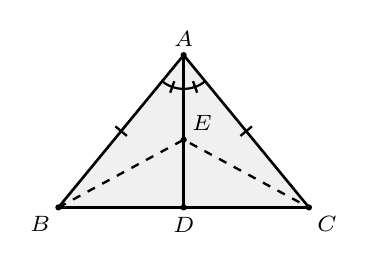
\begin{tikzpicture}[scale=0.86, every node/.style={font=\footnotesize, text=black}]
  \coordinate (A) at (0, 2.25);
  \coordinate (B) at (-1.85, 0);
  \coordinate (C) at (1.85, 0);
  \coordinate (D) at (0, 0);
  \coordinate (E) at (0, 1.00);
  \fill[gray!12] (A) -- (B) -- (C) -- cycle;
  \draw[black, line width=0.95pt] (B) -- (C);
  \draw[black, line width=0.95pt, tk1] (A) -- (B);
  \draw[black, line width=0.95pt, tk1] (A) -- (C);
  \draw[black, line width=1.15pt] (A) -- (D);
  \draw[black, line width=0.85pt, dashed] (B) -- (E) -- (C);
  \draw[black, line width=0.8pt] ($(A)+(-129.43:0.50)$) arc (-129.43:-50.57:0.50);
  \draw[black, line width=0.85pt] ($(A)+(-109.71:0.41)$) -- ($(A)+(-109.71:0.59)$);
  \draw[black, line width=0.85pt] ($(A)+(-70.29:0.41)$) -- ($(A)+(-70.29:0.59)$);
  \fill[black] (A) circle (1.3pt) node[above=2pt, inner sep=1pt] {$A$};
  \fill[black] (B) circle (1.3pt) node[below left=2pt, inner sep=1pt] {$B$};
  \fill[black] (C) circle (1.3pt) node[below right=2pt, inner sep=1pt] {$C$};
  \fill[black] (D) circle (1.3pt) node[below=2.5pt, inner sep=1pt] {$D$};
  \fill[black] (E) circle (1.3pt) node[above right=2pt, inner sep=1pt] {$E$};
\end{tikzpicture}}

% ២. រំលឹកទី១៖ ធ្នូរង្វង់ & គន្លងចម្ងាយថេរ
\newcommand{\figLocus}{%
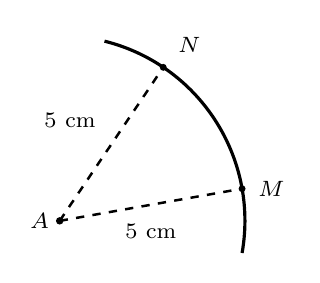
\begin{tikzpicture}[scale=0.96, every node/.style={font=\footnotesize, text=black}]
  \coordinate (A) at (0,0);
  \coordinate (P1) at (10:2.45);
  \coordinate (P2) at (56:2.45);
  \draw[black, line width=1.15pt] (A) ++(-10:2.45) arc (-10:76:2.45);
  \draw[black, line width=0.9pt, dashed] (A) -- (P1) node[midway, below=3pt] {$5\text{ cm}$};
  \draw[black, line width=0.9pt, dashed] (A) -- (P2) node[midway, above left=2pt] {$5\text{ cm}$};
  \fill[black] (A) circle (1.4pt) node[left=2.5pt, inner sep=1pt] {$A$};
  \fill[black] (P1) circle (1.3pt) node[right=2.5pt] {$M$};
  \fill[black] (P2) circle (1.3pt) node[above right=2pt] {$N$};
  \node at (33:3.05) {កាំថេរ};
\end{tikzpicture}}

% ៣. រំលឹកទី២៖ បូកអង្កត់ត្រង់ជួរ (F-J-G-K)
\newcommand{\figSegAdd}{%
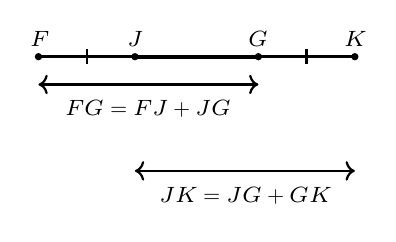
\begin{tikzpicture}[scale=0.98, every node/.style={font=\footnotesize, text=black}]
  \coordinate (F) at (0,0);
  \coordinate (J) at (1.25,0);
  \coordinate (G) at (2.85,0);
  \coordinate (K) at (4.10,0);
  \draw[black, line width=0.95pt, tk1] (F) -- (J);
  \draw[black, line width=1.45pt] (J) -- (G);
  \draw[black, line width=0.95pt, tk1] (G) -- (K);
  \foreach \p/\lbl in {F/$F$, J/$J$, G/$G$, K/$K$} {
    \fill[black] (\p) circle (1.35pt) node[above=2.5pt, inner sep=1pt] {\lbl};
  }
  \draw[black, line width=0.8pt, <->] (0,-0.36) -- (2.85,-0.36) node[midway, below=2pt] {$FG = FJ+JG$};
  \draw[black, line width=0.8pt, <->] (1.25,-1.48) -- (4.10,-1.48) node[midway, below=2pt] {$JK = JG+GK$};
\end{tikzpicture}}

% ៤. E1 Engage: អាថ៌កំបាំងគ្រោងដំបូលកំពង់ស្វាយ (៦, ៥, ៣ m) vs ស៊ុម ៤ របារ
\newcommand{\figRoofHook}{%
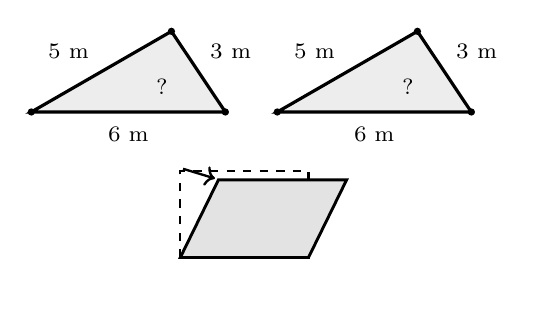
\begin{tikzpicture}[scale=0.88, every node/.style={font=\footnotesize, text=black}]
  % គ្រោងដំបូល ១ (6, 5, 3 m)
  \begin{scope}[shift={(0,0)}]
    \coordinate (A) at (0,0);
    \coordinate (B) at (2.80,0);
    \coordinate (C) at (2.022,1.164);
    \fill[gray!14] (A) -- (B) -- (C) -- cycle;
    \draw[black, line width=1.15pt] (A) -- (B) -- (C) -- cycle;
    \node[below=2pt] at ($(A)!0.5!(B)$) {$6\text{ m}$};
    \node[above left=1pt] at ($(A)!0.5!(C)$) {$5\text{ m}$};
    \node[above right=1pt] at ($(B)!0.5!(C)$) {$3\text{ m}$};
    \fill[black] (A) circle (1.5pt) (B) circle (1.5pt) (C) circle (1.5pt);
    \node at (1.75, 0.36) {មុំ?};
  \end{scope}
  % គ្រោងដំបូល ២ (6, 5, 3 m)
  \begin{scope}[shift={(3.55,0)}]
    \coordinate (Ap) at (0,0);
    \coordinate (Bp) at (2.80,0);
    \coordinate (Cp) at (2.022,1.164);
    \fill[gray!14] (Ap) -- (Bp) -- (Cp) -- cycle;
    \draw[black, line width=1.15pt] (Ap) -- (Bp) -- (Cp) -- cycle;
    \node[below=2pt] at ($(Ap)!0.5!(Bp)$) {$6\text{ m}$};
    \node[above left=1pt] at ($(Ap)!0.5!(Cp)$) {$5\text{ m}$};
    \node[above right=1pt] at ($(Bp)!0.5!(Cp)$) {$3\text{ m}$};
    \fill[black] (Ap) circle (1.5pt) (Bp) circle (1.5pt) (Cp) circle (1.5pt);
    \node at (1.75, 0.36) {ថេរ?};
  \end{scope}
  % ទ្វាររបង ៤ របារ (ទ្រេតដួល) ដាក់នៅជួរក្រោម
  \begin{scope}[shift={(2.15,-2.10)}]
    \draw[black, line width=0.8pt, dashed] (0,0) rectangle (1.85,1.25);
    \fill[gray!22] (0,0) -- (1.85,0) -- (2.40,1.12) -- (0.55,1.12) -- cycle;
    \draw[black, line width=1.05pt] (0,0) -- (1.85,0) -- (2.40,1.12) -- (0.55,1.12) -- cycle;
    \draw[black, line width=0.85pt, ->] (0.04,1.28) -- (0.50,1.14);
    \node[below=2.5pt] at (1.08,0) {៤ របារទ្រេត};
  \end{scope}
\end{tikzpicture}}

% ៥. E2 Explore Act 1: ស៊ុម ៤ របារទ្រេត vs ប្រសព្វធ្នូ ៦, ៥, ៣ cm ត្រង់ C
\newcommand{\figExploreOne}{%
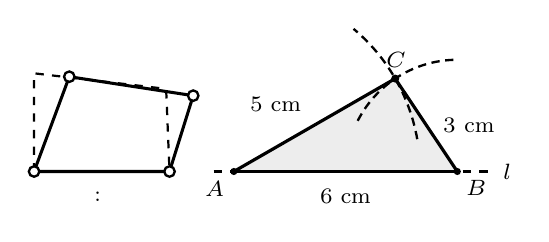
\begin{tikzpicture}[scale=0.86, every node/.style={font=\footnotesize, text=black}]
  % ឆ្វេង៖ ស៊ុម ៤ របារ (6, 5, 4, 3) ទ្រេត
  \begin{scope}[shift={(-2.90,0)}]
    \coordinate (P1) at (0,0);
    \coordinate (P2) at (2.00,0);
    \coordinate (P3) at (2.35,1.12);
    \coordinate (P4) at (0.52,1.40);
    \draw[black, line width=0.8pt, dashed] (P1) -- (0,1.45) -- (1.95,1.22) -- (P2);
    \draw[black, line width=1.1pt] (P1) -- (P2) -- (P3) -- (P4) -- cycle;
    \foreach \p in {P1,P2,P3,P4} {
      \fill[white, draw=black, line width=0.85pt] (\p) circle (2.2pt);
    }
    \node[below=4pt] at (1.05,0) {៤ របារ: មុំប្រែ};
  \end{scope}
  % ស្ដាំ៖ ធ្នូរង្វង់ប្រសព្វត្រង់ C (AB=6, AC=5, BC=3)
  \begin{scope}[shift={(0.05,0)}]
    \coordinate (A) at (0,0);
    \coordinate (B) at (3.30,0);
    \coordinate (C) at (2.383,1.372);
    \draw[black, line width=0.8pt, dashed] (-0.30,0) -- (3.75,0) node[right=2pt] {$l$};
    \fill[gray!14] (A) -- (B) -- (C) -- cycle;
    \draw[black, line width=1.15pt] (A) -- (B) node[midway, below=2.5pt] {$6\text{ cm}$};
    \draw[black, line width=1.15pt] (A) -- (C) node[midway, above left=1pt] {$5\text{ cm}$};
    \draw[black, line width=1.15pt] (B) -- (C) node[midway, right=2.5pt] {$3\text{ cm}$};
    \draw[black, line width=0.85pt, densely dashed] ($(A)+(10:2.75)$) arc (10:50:2.75);
    \draw[black, line width=0.85pt, densely dashed] ($(B)+(92:1.65)$) arc (92:154:1.65);
    \fill[black] (A) circle (1.5pt) node[below left=2pt, inner sep=1pt] {$A$};
    \fill[black] (B) circle (1.5pt) node[below right=2pt, inner sep=1pt] {$B$};
    \fill[black] (C) circle (1.7pt) node[above=2.5pt, inner sep=1pt] {$C$};
  \end{scope}
\end{tikzpicture}}

% ៦. E2 Explore Act 2: POE បដិឧទាហរណ៍ ម.ម.ម (4cm vs 6cm, 60°)
\newcommand{\figExploreAAA}{%
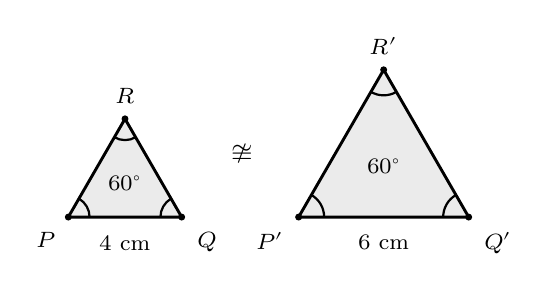
\begin{tikzpicture}[scale=0.90, every node/.style={font=\footnotesize, text=black}]
  % ត្រីកោណតូច 4 cm
  \coordinate (P) at (0,0);
  \coordinate (Q) at (1.60,0);
  \coordinate (R) at (0.80,1.386);
  \fill[gray!16] (P) -- (Q) -- (R) -- cycle;
  \draw[black, line width=1.05pt] (P) -- (Q) -- (R) -- cycle;
  \draw[black, line width=0.8pt] (0.30,0) arc (0:60:0.30);
  \draw[black, line width=0.8pt] (1.30,0) arc (180:120:0.30);
  \draw[black, line width=0.8pt] ($(R)+(-120:0.30)$) arc (-120:-60:0.30);
  \node at (0.80,0.48) {$60^\circ$};
  \node[below=3pt] at (0.80,0) {$4\text{ cm}$};
  \fill[black] (P) circle (1.4pt) node[below left=2pt] {$P$};
  \fill[black] (Q) circle (1.4pt) node[below right=2pt] {$Q$};
  \fill[black] (R) circle (1.4pt) node[above=2pt] {$R$};
  \node[font=\normalsize] at (2.45, 0.90) {$\not\cong$};
  % ត្រីកោណធំ 6 cm (មាត្រដ្ឋានដូចគ្នា 2:3)
  \begin{scope}[shift={(3.25,0)}]
    \coordinate (Pp) at (0,0);
    \coordinate (Qp) at (2.40,0);
    \coordinate (Rp) at (1.20,2.078);
    \fill[gray!16] (Pp) -- (Qp) -- (Rp) -- cycle;
    \draw[black, line width=1.05pt] (Pp) -- (Qp) -- (Rp) -- cycle;
    \draw[black, line width=0.8pt] (0.36,0) arc (0:60:0.36);
    \draw[black, line width=0.8pt] (2.04,0) arc (180:120:0.36);
    \draw[black, line width=0.8pt] ($(Rp)+(-120:0.36)$) arc (-120:-60:0.36);
    \node at (1.20,0.72) {$60^\circ$};
    \node[below=3pt] at (1.20,0) {$6\text{ cm}$};
    \fill[black] (Pp) circle (1.4pt) node[below left=2pt] {$P'$};
    \fill[black] (Qp) circle (1.4pt) node[below right=2pt] {$Q'$};
    \fill[black] (Rp) circle (1.4pt) node[above=2pt] {$R'$};
  \end{scope}
\end{tikzpicture}}

% ៧. E3 Explain: ទ្រឹស្ដីបទ ជ.ជ.ជ (SSS) – បង្វិល-ឆ្លុះ ~135° & កំពូលឈមជ្រុងស្មើ
\newcommand{\figThmSSS}{%
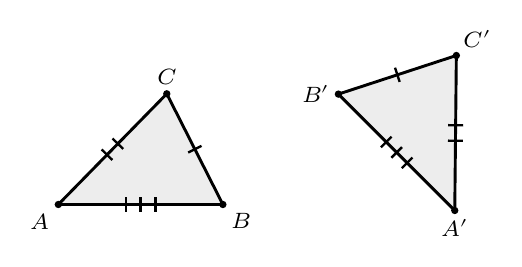
\begin{tikzpicture}[scale=0.95, every node/.style={font=\footnotesize, text=black}]
  \coordinate (A) at (0,0);
  \coordinate (B) at (2.20,0);
  \coordinate (C) at (1.45,1.48);
  \fill[gray!14] (A) -- (B) -- (C) -- cycle;
  \draw[black, line width=1.05pt, tk3] (A) -- (B);
  \draw[black, line width=1.05pt, tk2] (A) -- (C);
  \draw[black, line width=1.05pt, tk1] (B) -- (C);
  \fill[black] (A) circle (1.4pt) node[below left=2pt, inner sep=1pt] {$A$};
  \fill[black] (B) circle (1.4pt) node[below right=2pt, inner sep=1pt] {$B$};
  \fill[black] (C) circle (1.4pt) node[above=2pt, inner sep=1pt] {$C$};
  % ត្រីកោណទី២ ឆ្លុះ និងបង្វិល 135°
  \coordinate (Ap) at (5.30,-0.08);
  \coordinate (Bp) at (3.7444,1.4756);
  \coordinate (Cp) at (5.3212,1.9918);
  \fill[gray!14] (Ap) -- (Bp) -- (Cp) -- cycle;
  \draw[black, line width=1.05pt, tk3] (Ap) -- (Bp);
  \draw[black, line width=1.05pt, tk2] (Ap) -- (Cp);
  \draw[black, line width=1.05pt, tk1] (Bp) -- (Cp);
  \fill[black] (Ap) circle (1.4pt) node[below=2pt, inner sep=1pt] {$A'$};
  \fill[black] (Bp) circle (1.4pt) node[left=2pt, inner sep=1pt] {$B'$};
  \fill[black] (Cp) circle (1.4pt) node[above right=1.5pt, inner sep=1pt] {$C'$};
\end{tikzpicture}}

% ៨. E4 Elaborate: លំហាត់គំរូ (ទំព័រ ១៥២ – F-J-G-K ដេក & ស្ពាន JG)
\newcommand{\figModel}{%
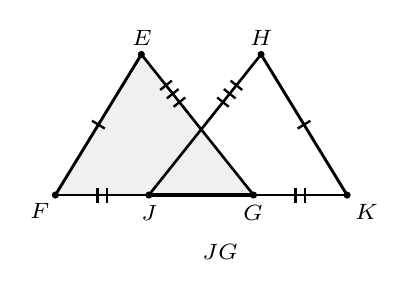
\begin{tikzpicture}[scale=0.95, every node/.style={font=\footnotesize, text=black}]
  \coordinate (F) at (0,0);
  \coordinate (J) at (1.25,0);
  \coordinate (G) at (2.65,0);
  \coordinate (K) at (3.90,0);
  \coordinate (E) at (1.15,1.88);
  \coordinate (H) at (2.75,1.88);
  \fill[gray!12] (E) -- (F) -- (G) -- cycle;
  \draw[black, line width=1.05pt, tk1] (E) -- (F);
  \draw[black, line width=1.05pt, tk1] (H) -- (K);
  \draw[black, line width=0.95pt, tk3u] (E) -- (G);
  \draw[black, line width=0.95pt, tk3u] (H) -- (J);
  \draw[black, line width=1.0pt, tk2] (F) -- (J);
  \draw[black, line width=1.0pt, tk2] (G) -- (K);
  \draw[black, line width=1.6pt] (J) -- (G);
  \fill[black] (F) circle (1.35pt) node[below left=2pt, inner sep=1pt] {$F$};
  \fill[black] (J) circle (1.35pt) node[below=2.5pt, inner sep=1pt] {$J$};
  \fill[black] (G) circle (1.35pt) node[below=2.5pt, inner sep=1pt] {$G$};
  \fill[black] (K) circle (1.35pt) node[below right=2pt, inner sep=1pt] {$K$};
  \fill[black] (E) circle (1.35pt) node[above=2pt, inner sep=1pt] {$E$};
  \fill[black] (H) circle (1.35pt) node[above=2pt, inner sep=1pt] {$H$};
  \node[below=14pt] at ($(J)!0.5!(G)$) {ស្ពាន $JG$};
\end{tikzpicture}}

% ៩. E5 Evaluate: លំហាត់ប្រតិបត្តិ (ទំព័រ ១៥៣ – R-S-T-V ឈរ & ស្ពាន ST)
\newcommand{\figPractice}{%
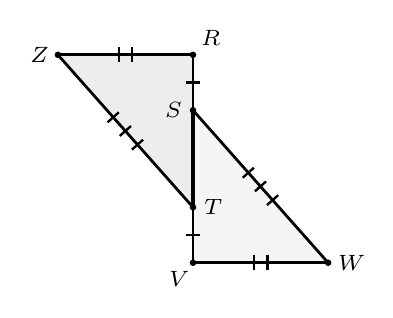
\begin{tikzpicture}[scale=0.88, every node/.style={font=\footnotesize, text=black}]
  \coordinate (R) at (0, 3.00);
  \coordinate (S) at (0, 2.20);
  \coordinate (T) at (0, 0.80);
  \coordinate (V) at (0, 0);
  \coordinate (Z) at (-1.95, 3.00);
  \coordinate (W) at (1.95, 0);
  \fill[gray!14] (R) -- (Z) -- (T) -- cycle;
  \fill[gray!8] (V) -- (W) -- (S) -- cycle;
  \draw[black, line width=1.05pt, tk2] (R) -- (Z);
  \draw[black, line width=1.05pt, tk2] (V) -- (W);
  \draw[black, line width=1.0pt, tk3] (Z) -- (T);
  \draw[black, line width=1.0pt, tk3] (S) -- (W);
  \draw[black, line width=1.05pt, tk1] (R) -- (S);
  \draw[black, line width=1.05pt, tk1] (T) -- (V);
  \draw[black, line width=1.6pt] (S) -- (T);
  \fill[black] (R) circle (1.35pt) node[above right=2pt, inner sep=1pt] {$R$};
  \fill[black] (S) circle (1.35pt) node[left=3pt, inner sep=1pt] {$S$};
  \fill[black] (T) circle (1.35pt) node[right=3pt, inner sep=1pt] {$T$};
  \fill[black] (V) circle (1.35pt) node[below left=2pt, inner sep=1pt] {$V$};
  \fill[black] (Z) circle (1.35pt) node[left=2.5pt, inner sep=1pt] {$Z$};
  \fill[black] (W) circle (1.35pt) node[right=2.5pt, inner sep=1pt] {$W$};
\end{tikzpicture}}

% ១០. E5 Evaluate: រូបសង្ខេបកាតត្រួតពិនិត្យ A-D (បំបែកជា ២ ជួរ 1x2 មិនឱ្យចង្អៀត ឬចន្លោះធំ)
\newcommand{\figExitCardsTop}{%
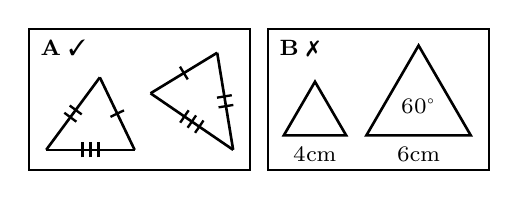
\begin{tikzpicture}[scale=0.92, every node/.style={font=\footnotesize, text=black}]
  % កាត A: SSS បង្វិល (~135 deg) ✓
  \begin{scope}[shift={(0,0)}]
    \draw[black, line width=0.85pt] (0,0) rectangle (3.05,1.95);
    \node[anchor=north west, inner sep=3pt] at (0.04,1.92) {\textbf{A} \ding{51}};
    \draw[black, line width=0.95pt, tk3] (0.24,0.28) -- (1.46,0.28);
    \draw[black, line width=0.95pt, tk2] (0.24,0.28) -- (0.98,1.28);
    \draw[black, line width=0.95pt, tk1] (1.46,0.28) -- (0.98,1.28);
    \draw[black, line width=0.95pt, tk3] (2.82,0.28) -- (1.68,1.06);
    \draw[black, line width=0.95pt, tk2] (2.82,0.28) -- (2.60,1.62);
    \draw[black, line width=0.95pt, tk1] (1.68,1.06) -- (2.60,1.62);
  \end{scope}
  % កាត B: AAA 60° (4cm vs 6cm) ✗
  \begin{scope}[shift={(3.30,0)}]
    \draw[black, line width=0.85pt] (0,0) rectangle (3.05,1.95);
    \node[anchor=north west, inner sep=3pt] at (0.04,1.92) {\textbf{B} \ding{55}};
    \draw[black, line width=0.95pt] (0.22,0.48) -- (1.08,0.48) -- (0.65,1.22) -- cycle;
    \node at (0.65,0.22) {$4\text{cm}$};
    \draw[black, line width=0.95pt] (1.36,0.48) -- (2.80,0.48) -- (2.08,1.72) -- cycle;
    \node at (2.08,0.88) {$60^\circ$};
    \node at (2.08,0.22) {$6\text{cm}$};
  \end{scope}
\end{tikzpicture}}

\newcommand{\figExitCardsBot}{%
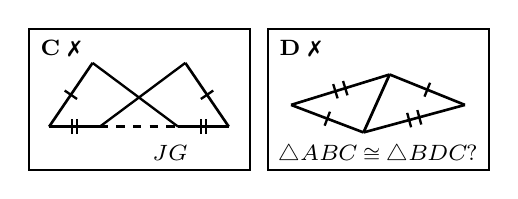
\begin{tikzpicture}[scale=0.92, every node/.style={font=\footnotesize, text=black}]
  % កាត C: FJ=GK ខ្វះស្ពាន JG ✗
  \begin{scope}[shift={(0,0)}]
    \draw[black, line width=0.85pt] (0,0) rectangle (3.05,1.95);
    \node[anchor=north west, inner sep=3pt] at (0.04,1.92) {\textbf{C} \ding{55}};
    \draw[black, line width=1.0pt, tk2] (0.28,0.60) -- (0.98,0.60);
    \draw[black, line width=1.0pt, tk2] (2.06,0.60) -- (2.76,0.60);
    \draw[black, line width=0.85pt, dashed] (0.98,0.60) -- (2.06,0.60);
    \draw[black, line width=0.95pt, tk1] (0.28,0.60) -- (0.88,1.48);
    \draw[black, line width=0.95pt, tk1] (2.76,0.60) -- (2.16,1.48);
    \draw[black, line width=0.85pt] (0.88,1.48) -- (2.06,0.60) (2.16,1.48) -- (0.98,0.60);
    \node at (1.52,0.24) {ខ្វះស្ពាន $JG$};
  \end{scope}
  % កាត D: លំដាប់កំពូលខុស ✗
  \begin{scope}[shift={(3.30,0)}]
    \draw[black, line width=0.85pt] (0,0) rectangle (3.05,1.95);
    \node[anchor=north west, inner sep=3pt] at (0.04,1.92) {\textbf{D} \ding{55}};
    \draw[black, line width=0.95pt, tk1] (0.32,0.90) -- (1.32,0.52);
    \draw[black, line width=0.95pt, tk1] (1.68,1.32) -- (2.72,0.90);
    \draw[black, line width=0.95pt, tk2] (0.32,0.90) -- (1.68,1.32);
    \draw[black, line width=0.95pt, tk2] (1.32,0.52) -- (2.72,0.90);
    \draw[black, line width=1.0pt] (1.32,0.52) -- (1.68,1.32);
    \node at (1.52,0.24) {$\tri{ABC}\cg\tri{BDC}$?};
  \end{scope}
\end{tikzpicture}}

% ១១. ជំហានទី៥ កិច្ចការផ្ទះ៖ លំហាត់ទី៤ (p.164) & លំហាត់ទី៩ (p.165)
\newcommand{\figHWnew}{%
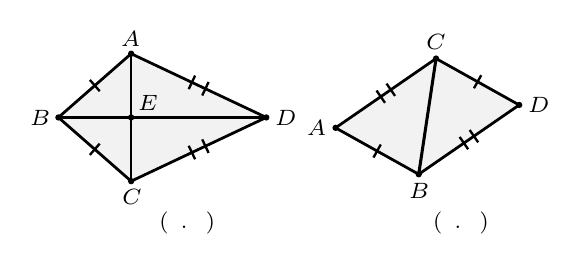
\begin{tikzpicture}[scale=0.88, every node/.style={font=\footnotesize, text=black}]
  % លំហាត់ទី៤ (ខ្លែង ABCD, E ប្រសព្វ AC, BD)
  \begin{scope}[shift={(-2.35,0)}]
    \coordinate (B) at (-1.05, 0);
    \coordinate (A) at (0, 0.92);
    \coordinate (C) at (0, -0.92);
    \coordinate (D) at (1.95, 0);
    \coordinate (E) at (0, 0);
    \fill[gray!10] (A) -- (B) -- (C) -- (D) -- cycle;
    \draw[black, line width=1.0pt, tk1] (A) -- (B);
    \draw[black, line width=1.0pt, tk1] (B) -- (C);
    \draw[black, line width=1.0pt, tk2] (A) -- (D);
    \draw[black, line width=1.0pt, tk2] (C) -- (D);
    \draw[black, line width=0.85pt] (A) -- (C) (B) -- (D);
    \fill[black] (A) circle (1.3pt) node[above=1.5pt, inner sep=1pt] {$A$};
    \fill[black] (B) circle (1.3pt) node[left=2pt, inner sep=1pt] {$B$};
    \fill[black] (C) circle (1.3pt) node[below=1.5pt, inner sep=1pt] {$C$};
    \fill[black] (D) circle (1.3pt) node[right=2pt, inner sep=1pt] {$D$};
    \fill[black] (E) circle (1.3pt) node[above right=1.5pt, inner sep=0.8pt] {$E$};
    \node at (0.35,-1.52) {លំហាត់ទី៤ (ទំ.១៦៤)};
  \end{scope}
  % លំហាត់ទី៩ (ចតុកោណ ABDC, BC រួម)
  \begin{scope}[shift={(1.75,0)}]
    \coordinate (A) at (-1.15, -0.15);
    \coordinate (B) at (0.05, -0.82);
    \coordinate (C) at (0.30, 0.85);
    \coordinate (D) at (1.50, 0.18);
    \fill[gray!10] (A) -- (B) -- (D) -- (C) -- cycle;
    \draw[black, line width=1.0pt, tk1] (A) -- (B);
    \draw[black, line width=1.0pt, tk1] (C) -- (D);
    \draw[black, line width=1.0pt, tk2] (A) -- (C);
    \draw[black, line width=1.0pt, tk2] (B) -- (D);
    \draw[black, line width=1.1pt] (B) -- (C);
    \fill[black] (A) circle (1.3pt) node[left=2pt, inner sep=1pt] {$A$};
    \fill[black] (B) circle (1.3pt) node[below=2pt, inner sep=1pt] {$B$};
    \fill[black] (C) circle (1.3pt) node[above=2pt, inner sep=1pt] {$C$};
    \fill[black] (D) circle (1.3pt) node[right=2pt, inner sep=1pt] {$D$};
    \node at (0.20,-1.52) {លំហាត់ទី៩ (ទំ.១៦៥)};
  \end{scope}
\end{tikzpicture}}

% ============================================================================
% ចាប់ផ្ដើមឯកសារ (Document Body)
% ============================================================================
\begin{document}
\fontsize{10pt}{15.2pt}\selectfont

% -------------------- ក្បាលកិច្ចតែងការ (Header) --------------------
\begin{center}
  {\muol\fontsize{11pt}{16pt}\selectfont ព្រះរាជាណាចក្រកម្ពុជា}\\[1pt]
  {\muol\fontsize{10pt}{15pt}\selectfont ជាតិ សាសនា ព្រះមហាក្សត្រ}\\[0pt]
  \khmflourish
\end{center}

\vspace{-22pt}
{\muol\fontsize{9.5pt}{13.0pt}\selectfont
មន្ទីរអប់រំ យុវជន និងកីឡា ខេត្តកំពង់ធំ\\
ការិយាល័យអប់រំ យុវជន និងកីឡា ស្រុកកំពង់ស្វាយ\\
អនុវិទ្យាល័យព្រះក្រសាំង}

\vspace{0pt}
\begin{center}
  {\muol\fontsize{10pt}{15pt}\selectfont កិច្ចតែងការបង្រៀន}
\end{center}
\vspace{0pt}

% -------------------- ព័ត៌មានទូទៅ (Metadata) --------------------
{\renewcommand{\arraystretch}{0.92}
\hspace*{4.6cm}%
\begin{tabular}{@{}l l l@{}}
  - \hspace{0.35cm} មុខវិជ្ជា & : & គណិតវិទ្យា ថ្នាក់ទី៨ \\
  - \hspace{0.35cm} ចំណងជើងមេរៀន & : & មេរៀនទី១២ ការប្រៀបធៀបត្រីកោណ \\
  - \hspace{0.35cm} ចំណងជើងរង & : & ១.២. លក្ខខណ្ឌនៃត្រីកោណប៉ុនគ្នា \\
  & & ១.២.៣ ជ្រុងបីប៉ុនរៀងគ្នា (ជ.ជ.ជ) \\
  - \hspace{0.35cm} រយៈពេល & : & ១ ម៉ោងសិក្សា (៥០នាទី) \\
  - \hspace{0.35cm} បង្រៀនដោយ & : & ហុក ប៊ុនថែន \\
  - \hspace{0.35cm} កាលបរិច្ឆេទ & : & ថ្ងៃសុក្រ ទី២៧ ខែវិច្ឆិកា ឆ្នាំ២០២៦ \\
\end{tabular}

\vspace{0pt}

% -------------------- I. វត្ថុបំណង --------------------
\textbf{I.} {\muol វត្ថុបំណង}\\[1pt]
\hspace*{0.55cm}%
\begin{tabular}{@{}l l l@{}}
  \wcirc \hspace{0.25cm} វិជ្ជាសម្បទា & : & សិស្សកំណត់បានពីលក្ខខណ្ឌត្រីកោណពីរប៉ុនគ្នាករណី ជ្រុងបីប៉ុនរៀងគ្នា (ជ.ជ.ជ) តាមពិសោធន៍ស៊ុម ៣ របារ \\
  & & ធៀបនឹង ៤ របារ ការសង់ប្រសព្វធ្នូដែកឈាន និងបដិសេធបានត្រឹមត្រូវនូវអន្ទាក់ ម.ម.ម (AAA) ។ \\
  \wcirc \hspace{0.25cm} បំណិនសម្បទា & : & សិស្សបកស្រាយ និងស្រាយបញ្ជាក់ត្រីកោណត្រួតគ្នាដោយប្រើ «ស្ពានតភ្ជាប់អង្កត់ និងគំនូស $|, \parallel, |||$» \\
  & & គោលការណ៍កំពូលឈមជ្រុងស្មើ និងធនាគារហេតុផល \cnum{1}--\cnum{5} ដើម្បីដោះស្រាយបញ្ហាគ្រោងដំបូល និងលំហាត់ ។ \\
  \wcirc \hspace{0.25cm} ចរិយាសម្បទា & : & សិស្សសហការជា «ក្រុមជាងសំណង់ដំបូល» ហ៊ានទស្សន៍ទាយ ពិសោធន៍ផ្ទាល់ដៃ និងផ្ទៀងផ្ទាត់កំហុស \\
  & & ដោយស្មារតីទទួលខុសត្រូវ និងយុត្តិធម៌ ។ \\
\end{tabular}

\vspace{0pt}

% -------------------- II. សម្ភារៈឧបទេស --------------------
\textbf{II.} {\muol សម្ភារៈឧបទេស}\\[1pt]
\hspace*{0.55cm}$\bullet$ \hspace{0.35cm} សៀវភៅគោលទី៨ ដែកឈាន បន្ទាត់ កញ្ចប់កាត់ ១:១ (របារ $6,5,4,3\text{cm}$ \& ត្រីកោណ AAA $4,6\text{cm}$) កាតសកម្មភាព E4--E5 \& កាត A--D (ស-ខ្មៅ)

\vspace{0pt}

% -------------------- III. វិធីសាស្រ្តបង្រៀន --------------------
\textbf{III.} {\muol វិធីសាស្រ្តបង្រៀន}\\[1pt]
\hspace*{0.55cm}%
\begin{tabular}{@{}l l l@{}}
  $\bullet$ \hspace{0.35cm} គោលវិធី & : \hspace{0.7cm} & សិស្សមជ្ឈមណ្ឌល \\
  $\bullet$ \hspace{0.35cm} យុទ្ធវិធីបង្រៀន & : & ស្ថាបនានិយម គម្រូ 5Es (ពិសោធន៍ស៊ុមរឹង POE ស្ពានអង្កត់ \textbf{[tracing]} \& អធិការកិច្ច ៣ តួនាទី) \\
\end{tabular}
}

\vspace{0pt}

% -------------------- IV. ដំណើរការបង្រៀន --------------------
\textbf{IV.} {\muol ដំណើរការបង្រៀន}

\vspace{0pt}

% ============================================================================
% តារាងដំណើរការបង្រៀន (Granular Sub-Row 3-Column Table – 50 នាទី)
% ============================================================================
\renewcommand{\arraystretch}{1.15}
\begin{longtable}{|L{5.50cm}|L{7.90cm}|L{4.80cm}|}
\hline
\rowcolor{headgray}
\multicolumn{1}{|c|}{\muol សកម្មភាពគ្រូ} &
\multicolumn{1}{c|}{\muol ខ្លឹមសារមេរៀន} &
\multicolumn{1}{c|}{\muol សកម្មភាពសិស្ស} \\
\hline
\endfirsthead

\hline
\endhead

\hline
\endfoot

\hline
\endlastfoot

% ==================== ជំហានទី១ (2min) ====================
\stepheader{ជំហានទី១ (រដ្ឋបាលថ្នាក់)}
- ពិនិត្យអវត្តមាន និងអនាម័យថ្នាក់រៀន \par
- ចាត់សិស្សជាក្រុម ៣ នាក់ («ក្រុមជាងសំណង់ដំបូល») និងចែកកញ្ចប់សម្ភារៈកាត់ ១:១ (ស-ខ្មៅ) ទុកលើតុ
&
\hspace*{0.3cm}- រដ្ឋបាលថ្នាក់ \par
\hspace*{0.3cm}- អនាម័យ និងសណ្ដាប់ធ្នាប់ថ្នាក់រៀន \par
\hspace*{0.3cm}- ត្រៀមក្រុមជាងសំណង់ដំបូល
&
- រាយការណ៍អវត្តមាន \par
- រៀបចំតុតាមក្រុម ៣ នាក់ \\
\hline

% ==================== ជំហានទី២ (9min: HW <=3m + Prereq <=3m + E1 3m) ====================
\stepheader{ជំហានទី២ (កិច្ចការផ្ទះ + ទំនាក់ទំនងមេរៀនថ្មី)}
% --- ២.១a កំណែកិច្ចការផ្ទះ៖ ល្បែងចាប់កំហុស ---
\timenote{(កំណែកិច្ចការផ្ទះ៖ មិនឱ្យលើស 3min)} \par
- ពិនិត្យកិច្ចការផ្ទះសិស្សជាមុន \par
\ditem \textbf{ល្បែងចាប់កំហុស} ៖ \par
– សំណួរ៖ តើអាចយក $AB=AC$ មកដាក់ក្នុង $\tri{BDE}$ និង $\tri{CDE}$ បានឬទេ? ហេតុអ្វី?
&
\centerline{\redsub{កំណែកិច្ចការផ្ទះ (មេរៀនមុន ម.ជ.ម)}} \par
\hspace*{0.1cm}$\tri{ABC}$ ($AB=AC$), កន្លះបន្ទាត់ពុះ $AD$ ($D\in BC$), $E\in AD$ ។
&
- ផ្ទៀង និងឆ្លើយ៖ «ទេ! $AB, AC$ មិនមែនជ្រុងនៃ $\tri{BDE}, \tri{CDE}$ ទេ» \\[3pt]

% --- ២.១b រូបភាពកំណែកិច្ចការផ្ទះ (Isolated Row) ---
&
\cfig{\figHWold}
&
\\[3pt]

% --- ២.២a ចម្លើយកិច្ចការផ្ទះ (ក) ---
- បង្ហាញចម្លើយសង្ខេបផ្នែក ក និងសង្កត់ធ្ងន់លើធាតុមូលដ្ឋាន ម.ជ.ម
&
\centerline{\underline{ចម្លើយ}} \par
ក. ក្នុង $\tri{ABD}$ និង $\tri{ACD}$ មាន៖ \par
\hspace*{0.3cm}$AB=AC$ (បម្រាប់) \par
\hspace*{0.3cm}$\ang{BAD}=\ang{CAD}$ ($AD$ ពុះមុំ) \par
\hspace*{0.3cm}$AD=AD$ (ជ្រុងរួម) \par
\hspace*{0.2cm}$\Rightarrow \tri{ABD} \cg \tri{ACD}$ (ម.ជ.ម) \par
\hspace*{0.2cm}+ វិបាក៖ $DB=DC$ និង $\ang{ADB}=\ang{ADC}$
&
- ផ្ទៀងផ្ទាត់សមភាព និងហេតុផលផ្នែក ក \\[3pt]

% --- ២.២b ចម្លើយកិច្ចការផ្ទះ (ខ) ---
- សង្កត់ធ្ងន់ការបញ្ជូន $DB=DC$ និង $\ang{ADB}=\ang{ADC}$ ពី ក ទៅ ខ
&
ខ. ក្នុង $\tri{BDE}$ និង $\tri{CDE}$ មាន៖ \par
\hspace*{0.3cm}$BD=CD$ (វិបាក ក) \par
\hspace*{0.3cm}$\ang{BDE}=\ang{CDE}$ (វិបាក ក) \par
\hspace*{0.3cm}$DE=DE$ (ជ្រុងរួម) \par
\hspace*{0.2cm}$\Rightarrow$ \graybox{$\tri{BDE} \cg \tri{CDE}$ (ម.ជ.ម) $\Rightarrow EB=EC$}
&
- ផ្ទៀងផ្ទាត់តាមលំដាប់ ក $\rightarrow$ ខ \\[3pt]

% --- ២.៣a រំលឹកទី១៖ ធ្នូរង្វង់ & គន្លងចម្ងាយថេរ ---
\timenote{(រំលឹកមេរៀន៖ រួម ២ ភាគមិនឱ្យលើស 3min)} \par
\ditem \textbf{រំលឹករហ័ស (ភាគ ១)} ៖ គូសធ្នូកាំ $5\text{cm}$ ផ្ចិត $A$ \par
– សំណួរ៖ តើចំណុចលើធ្នូមានចម្ងាយប៉ុន្មានពី $A$?
&
\centerline{\redsub{រំលឹកមេរៀនទាក់ទងមេរៀនថ្មី}} \par
\hspace*{0.1cm}- \textbf{ធ្នូរង្វង់ និងគន្លងចម្ងាយថេរ} (\graybox{\textit{Compass Locus}})
&
- ឆ្លើយស្រុះ៖ «គ្រប់ចំណុចលើធ្នូមានចម្ងាយ $5\text{cm}$ ពី $A$» \\[3pt]

% --- ២.៣b រូបភាពធ្នូរង្វង់ (Isolated Row) ---
&
\cfig{\figLocus}
\centerline{គ្រប់ចំណុចលើធ្នូផ្ចិត $A$ កាំ $5\text{cm}$ មានចម្ងាយ $5\text{cm}$ ពី $A$}
&
\\[3pt]

% --- ២.៤a រំលឹកទី២៖ បូកអង្កត់ត្រង់ជួរ ---
\ditem \textbf{រំលឹករហ័ស (ភាគ ២)} ៖ បង្ហាញ $F\text{-}J\text{-}G\text{-}K$ រត់ត្រង់ជួរ \par
– សំណួរ៖ បើ $FJ=GK$ តើ $FG$ និង $JK$ យ៉ាងណា?
&
\hspace*{0.1cm}- \textbf{ការបូកអង្កត់ត្រង់ជួរ} (\graybox{\textit{Collinear Segment Addition}})
&
- សង្កេតអង្កត់រួម $JG$ \par
- ឆ្លើយ៖ «$FG = JK$» \\[3pt]

% --- ២.៤b រូបភាពបូកអង្កត់ត្រង់ជួរ (Isolated Row) ---
&
\cfig{\figSegAdd}
\centerline{បើ $FJ=GK \Rightarrow FG = FJ+JG = GK+JG = JK$}
&
\\[3pt]

% --- ២.៥a E1 Engage: អាថ៌កំបាំងគ្រោងដំបូលកំពង់ស្វាយ ---
\fiveE{E1 - Engage} \timenote{(3min)} \par
\ditem \textbf{អាថ៌កំបាំងគ្រោងដំបូលឈើ និងស្ពានដែក} ៖ \par
ជាង ២ នាក់នៅកំពង់ស្វាយកាត់ឈើគ្រោងដំបូល $6\text{m}, 5\text{m}, 3\text{m}$ ដូចគ្នា ដោយ \textbf{គ្មានរ៉ាព័រទ័រវាស់មុំ} ។
&
\centerline{\redsub{ស្ថានភាពបញ្ហាពិត៖ គ្រោងដំបូលឈើ ($6\text{ m}, 5\text{ m}, 3\text{ m}$)}}
&
- សង្កេតភាពរឹងមាំគ្រោងដំបូល vs ទ្វារ ៤ របារ \\[3pt]

– សំណួរ៖ ហេតុអ្វីដំបូលទាំងពីរចាក់សោបានមុំនិងរាងដូចគ្នា ខណៈទ្វារ ៤ របារទ្រេតដួល?
&
&
- ទស្សន៍ទាយមូលហេតុ \\[3pt]

% --- ២.៥b រូបភាពគ្រោងដំបូល (Isolated Row) ---
&
\cfig{\figRoofHook}
&
\\[3pt]

% --- ២.៥c សំណួរចោទបញ្ចប់ E1 ---
- សង្កត់ធ្ងន់បញ្ហាគន្លឹះដើម្បីទាញចូលការពិសោធន៍
&
\textbf{ចម្ងល់} ៖ គ្មានរ៉ាព័រទ័រ តើស្គាល់តែ ៣ ជ្រុងគ្រប់គ្រាន់ឱ្យ $\tri{ABC}\cg\tri{A'B'C'}$ ឬទេ?
&
- ចង់ពិសោធន៍ផ្ទាល់ដៃជាមួយស៊ុម ៣ របារ និង ៤ របារ \\
\hline

% ==================== ជំហានទី៣ (17min: E2 11m + E3 6m) ====================
\stepheader{ជំហានទី៣ (ខ្លឹមសារមេរៀនថ្មី)}
% --- ៣.១a ចំណងជើង & E2 Act 1 (7min) ---
\fiveE{E2 - Explore} \timenote{(11min)} \par
- សរសេរចំណងជើងមេរៀនលើក្ដារខៀន \par
\ditem \textbf{សកម្មភាព ១៖ ស៊ុម ៤ vs ៣ របារ \& ប្រសព្វធ្នូ} \timenote{(7min)} \par
+ តភ្ជាប់របារ $6,5,4,3\text{cm}$ (៤ របារ) រុញចុះឡើង \par
+ តភ្ជាប់ $AB=6, AC=5, BC=3\text{cm}$ និងគូសធ្នូកាំ $r_1=5\text{cm}$ ($A$), $r_2=3\text{cm}$ ($B$) លើក្រដាស ១:១
&
មេរៀនទី១២ \hspace{0.15cm} {\muol ការប្រៀបធៀបត្រីកោណ (ត)} \par
១.២. លក្ខខណ្ឌនៃត្រីកោណប៉ុនគ្នា \par
១.២.៣ ជ្រុងបីប៉ុនរៀងគ្នា (ជ.ជ.ជ)
&
- កត់ចំណងជើង \par
- តេស្តស៊ុម ៤ vs ៣ របារ \par
- គូសប្រសព្វធ្នូត្រង់ $C$ \\[3pt]

% --- ៣.១b រូបភាពពិសោធន៍សកម្មភាព ១ (Isolated Row) ---
&
\cfig{\figExploreOne}
&
\\[3pt]

% --- ៣.១c សង្កេត និងផ្ទៀងត្រួត ---
+ ឱ្យសិស្សបង្វិល-ត្រឡប់ក្រដាសត្រីកោណផ្ទៀងត្រួតលើក្រុមជិតខាង
&
+ ៤ របារ៖ រាងប្រែសេរី \par
+ ៣ របារ ($6,5,3\text{cm}$)៖ ធ្នូ $r_1, r_2$ ប្រសព្វត្រង់ $C$ តែ \textbf{១ គត់} $\rightarrow$ ត្រួតបង្វិល-ត្រឡប់ស៊ីគ្នា ១០០\%!
&
- យកក្រដាសកាត់ផ្ទៀងត្រួតលើក្រុមជិតខាង \\[3pt]

% --- ៣.២a E2 Act 2 (4min): POE AAA + 2, 2.5, 6 cm ---
\ditem \textbf{សកម្មភាព ២៖ POE អន្ទាក់ ម.ម.ម} \timenote{(4min)} \par
+ \textbf{ទស្សន៍ទាយ (P)}៖ $\tri{PQR}$ ($4\text{cm}$) និង $\tri{P'Q'R'}$ ($6\text{cm}$) មានមុំ $60^\circ$ ដូចគ្នាទាំង ៣ — តើប៉ុនគ្នាឬ? \par
+ \textbf{សង្កេត-ពន្យល់ (O-E)}៖ យកកាត់ ១:១ ដាក់ត្រួតលើគ្នា រួចតេស្តបន្ទះ $2, 2.5, 6\text{cm}$
&
\centerline{\textbf{បដិឧទាហរណ៍ ម.ម.ម (AAA) \& របារមិនប្រសព្វ}}
&
- ទស្សន៍ទាយមុន \par
- ដាក់ត្រួតកាត់ $4\text{cm}$ vs $6\text{cm}$ ច្រានចោល ម.ម.ម \\[3pt]

% --- ៣.២b រូបភាពបដិឧទាហរណ៍ ម.ម.ម (Isolated Row) ---
&
\cfig{\figExploreAAA}
&
\\[3pt]

% --- ៣.២c សង្ខេបបដិឧទាហរណ៍ ---
- បញ្ជាក់លក្ខខណ្ឌមិនបង្កើតបានត្រីកោណ ($2+2.5 < 6$)
&
\graybox{$\tri{PQR} \ncg \tri{P'Q'R'}$ (ម.ម.ម មិនប៉ុនគ្នា)} \par
$2+2.5=4.5<6$ (របារមិនប្រសព្វគ្នា)
&
- តេស្តបន្ទះ $2, 2.5, 6\text{cm}$ និងទាញសេចក្ដីសន្និដ្ឋាន \\[3pt]

% --- ៣.៣a1 E3 Explain: ទ្រឹស្ដីបទ ជ.ជ.ជ ---
\fiveE{E3 - Explain} \timenote{(6min)} \par
\ditem នាំសិស្សបង្គុំទ្រឹស្ដីបទ ជ.ជ.ជ
&
\textbf{ទ្រឹស្ដីបទ (ជ.ជ.ជ) ៖} ត្រីកោណពីរប៉ុនគ្នា កាលណាវាមានជ្រុងទាំងបីប៉ុនរៀងគ្នា ។
&
- បង្គុំទ្រឹស្ដីបទ ជ.ជ.ជ \\[3pt]

% --- ៣.៣a2 គោលការណ៍កំពូលឈមជ្រុងស្មើ ---
– សំណួរ \cnum{1}៖ តើផ្គូផ្គងកំពូលលើរូបបង្វិល-ឆ្លុះ $\approx 135^\circ$ ដូចម្ដេច?
&
\redsub{\textbf{គោលការណ៍កំពូលឈមជ្រុងស្មើ} ៖} ផ្គូផ្គងកំពូលឈមនឹងជ្រុងគំនូសស្មើ ($|$ ឈម $A\leftrightarrow A'$, $\parallel$ ឈម $B\leftrightarrow B'$, $|||$ ឈម $C\leftrightarrow C'$) ។
&
- អនុវត្តគោលការណ៍កំពូលឈមជ្រុងស្មើ \\[3pt]

% --- ៣.៣b រូបភាពទ្រឹស្ដីបទ ជ.ជ.ជ (Isolated Row) ---
&
\cfig{\figThmSSS}
&
\\[3pt]

% --- ៣.៤a E3 Explain: តារាងកែតម្រូវ BC=B'C' (Isolated Row) ---
– សំណួរ \cnum{2}៖ ផ្ទៀងតារាងសៀវភៅទំព័រ ១៥២៖ «តើជួរទី ៣ ក្រោមសម្មតិកម្មត្រូវជាអ្វី?» + ធនាគារហេតុផល \cnum{1}--\cnum{5}
&
\cfig{%
\setlength{\tabcolsep}{2.2pt}%
\renewcommand{\arraystretch}{1.12}%
\begin{tabular}{|c|c|c|}
  \hline
  \cellcolor{headgray} សម្មតិកម្ម (ជ.ជ.ជ) & \cellcolor{headgray} សន្និដ្ឋាន & \cellcolor{headgray} វិបាក \\
  \hline
  $AB = A'B'$ & & $\ang{A} = \ang{A'}$ \\
  $AC = A'C'$ & $\tri{ABC} \cg \tri{A'B'C'}$ & $\ang{B} = \ang{B'}$ \\
  \textbf{$BC = B'C'$} {\footnotesize (កែពី $AB$)} & {\footnotesize (តាមលក្ខខណ្ឌ ជ.ជ.ជ)} & $\ang{C} = \ang{C'}$ \\[2pt]
  \hline
\end{tabular}%
}
&
- រកឃើញ និងកែ \textbf{$BC=B'C'$} (ទំព័រ ១៥២) \\[3pt]

% --- ៣.៤b ធនាគារហេតុផល ①–⑤ & សម្គាល់ = vs \cong ---
- សង្ខេបធនាគារហេតុផល \cnum{1}--\cnum{5} និងភាពខុសគ្នា $=$ vs $\cg$
&
\textbf{ធនាគារហេតុផល៖} \par
\cnum{1} បម្រាប់ \quad \cnum{2} បូក/ដកអង្កត់រួម ($FJ+JG$ / $RS+ST$) \par
\cnum{3} ជ្រុងរួម \quad \cnum{4} ជ.ជ.ជ $\rightarrow$ \cnum{5} ធាតុត្រូវគ្នា (មុំឈមជ្រុងស្មើ) ។ \par
\textbf{សម្គាល់}៖ $=$ (ប្រវែង/រង្វាស់ស្មើគ្នា) និង $\cg$ (ត្រីកោណប៉ុនគ្នា) ។
&
- កត់ \cnum{1}--\cnum{5} និង $=$ vs $\cg$ \\
\hline

% ==================== ជំហានទី៤ (20min: E4 10m + E5 10m) ====================
\stepheader{ជំហានទី៤ (ពង្រីកចំណេះដឹង)}
% --- ៤.១a E4 Elaborate: លំហាត់គំរូ F-J-G-K & ស្ពាន JG ---
\fiveE{E4 - Elaborate} \timenote{(10min)} \par
\ditem ចែកកាត \textbf{«ស្ពានតភ្ជាប់អង្កត់ $JG$ និងគំនូស $|, \parallel, |||$»} (ទំព័រ ២) ប្រើម្រាមដៃ \textbf{[tracing]}៖ \par
\cnum{1} អូស + គូស $|$ ($EF=HK$), $\parallel$ ($FJ=GK$), $|||$ ($EG=HJ$) \par
\cnum{2} អូសស្ពានរួម $JG$ តភ្ជាប់ $FG = JK$ \par
\cnum{3} ផ្គូផ្គង ៣ ជ្រុង $\rightarrow$ \cnum{4} $\rightarrow$ វិបាក \cnum{5}
&
{\muol លំហាត់គំរូ (ទំព័រ ១៥២)} \textbf{:} ក្នុងរូប $F\text{-}J\text{-}G\text{-}K$ រត់ត្រង់ជួរ គេឱ្យ $EF=HK$, $FJ=GK$ និង $EG=HJ$ ។ \par
\hspace*{0.2cm}ក. បង្ហាញថា $\tri{EFG} \cg \tri{HKJ}$ ។ \par
\hspace*{0.2cm}ខ. ទាញបញ្ជាក់ថា $\ang{E} = \ang{H}$ ។
&
- អូសម្រាមដៃ \textbf{[tracing]} គូស $|, \parallel, |||$ និងអូសស្ពាន $JG$ លើកាត \\[3pt]

% --- ៤.១b រូបភាពលំហាត់គំរូ (Isolated Row) ---
&
\cfig{\figModel}
&
\\[3pt]

% --- ៤.២a ចម្លើយលំហាត់គំរូ (ក) ---
\ditem ដឹកនាំសរសេរភស្តុតាង \cnum{1}--\cnum{4} ផ្នែក ក
&
\centerline{\underline{\redsub{ចម្លើយ (ស្ពាន $JG$ \& ហេតុផល \cnum{1}--\cnum{5})}}} \par
ក. ដោយ $FJ=GK$ (\cnum{1}) នោះ \par
\hspace*{0.30cm}$FG = FJ+JG = GK+JG = JK$ (\cnum{2} បូក $JG$) \par
\hspace*{0.15cm}ក្នុង $\tri{EFG}$ និង $\tri{HKJ}$ មាន៖ \par
\hspace*{0.30cm}$EF=HK$ (\cnum{1} បម្រាប់) \par
\hspace*{0.30cm}$EG=HJ$ (\cnum{1} បម្រាប់) \par
\hspace*{0.30cm}$FG=JK$ (\cnum{2} ស្រាយខាងលើ) \par
\hspace*{0.20cm}$\Rightarrow$ \graybox{$\tri{EFG}\cg\tri{HKJ}$ (\cnum{4} ជ.ជ.ជ)}
&
- បំពេញកាត \cnum{1}--\cnum{4} ជាមួយដៃគូ \\[3pt]

% --- ៤.២b ចម្លើយលំហាត់គំរូ (ខ) ---
\ditem នាំទាញវិបាក (ខ) ពីភាពប៉ុនគ្នា
&
ខ. វិបាក \cnum{5}៖ ដោយ $\tri{EFG}\cg\tri{HKJ}$ \par
\hspace*{0.20cm}$\Rightarrow$ \graybox{$\ang{E}=\ang{H}$} (មុំឈមនឹង $FG=JK$)
&
- ទាញវិបាក $\ang{E}=\ang{H}$ \\[3pt]

% --- ៤.២c EIA ពិនិត្យក្រោយ (30s) ---
\ditem សួរ \textbf{EIA ពិនិត្យក្រោយ (30s)}៖ \par
«បើរំកិល $\tri{HKJ}$ តាមបន្ទាត់ $FK$ ដោយរក្សា $FJ=GK$ តើអ្វីប្រែ ($JG, FG, JK$) និងអ្វីថេរ ($FG=JK$)?»
&
\timenote{EIA 30s៖ ទោះ $JG, FG, JK$ ប្រែប្រវែង ក៏ $FG=JK$ និង $\tri{EFG}\cg\tri{HKJ}$ ថេរ!}
&
- ញែកអ្វីប្រែ vs អ្វីថេរពេលរំកិល $\tri{HKJ}$ \\[3pt]

% --- ៤.៣a E5 Evaluate: ប្រតិបត្តិ R-S-T-V ---
\fiveE{E5 - Evaluate} \timenote{(10min)} \par
\ditem {\muol លំហាត់ប្រតិបត្តិ (ទំព័រ ១៥៣)} \par
ប្រើសន្លឹក \textbf{«ក្រុមអធិការកិច្ចប្លង់ ៣ តួនាទី»} (ទំព័រ ៣) \textbf{(៣០វិ./ម្នាក់)}៖ \par
គេឱ្យ $R\text{-}S\text{-}T\text{-}V$ រត់ត្រង់ជួរឈរ, $RZ=VW$, $TZ=SW$, $RS=TV$ ។ ចូរប្រៀបធៀប $\tri{RZT}$ និង $\tri{VWS}$ រួច \textbf{បិទបញ្ហាដំបូល E1} ។
&
{\muol ចម្លើយលំហាត់ប្រតិបត្តិ} \par
ប្រៀបធៀប $\tri{RZT}$ និង $\tri{VWS}$
&
- អានប្រធាន និងបែងចែកតួនាទី ១--៣ \\[3pt]

% --- ៤.៣b រូបភាពលំហាត់ប្រតិបត្តិ (Isolated Row) ---
&
\cfig{\figPractice}
&
\\[3pt]

% --- ៤.៤a E5 Evaluate: ក្រុមអធិការកិច្ច វេន ១--២ (Pause-Ask & ស្ពាន ST) ---
- ចាត់វេនអធិការកិច្ច (\textbf{Pause-Ask} មុនគូស/ផ្ទេរវេន)៖ \par
\cnum{1} \textbf{អ្នកទី១ (Pause-Ask / គូស $|, \parallel, |||$)}៖ ពន្យល់មុនគូស $RZ=VW, TZ=SW, RS=TV$ (\textbf{ហាមគូស $RT=SV$ មុនតស្ពាន}) \par
\cnum{2} \textbf{អ្នកទី២ (តភ្ជាប់ \& \cnum{1}--\cnum{4})}៖ អូសស្ពានឈរ $ST$ រក $RT=SV$ សរសេរ ៣ បន្ទាត់ \cnum{1}--\cnum{4}
&
+ ស្ពានឈរ៖ ដោយ $RS=TV$ (\cnum{1}) នោះ \par
\hspace*{0.25cm}$RT = RS + ST = ST + TV = SV$ (\cnum{2} បូក $ST$) \par
+ ក្នុង $\tri{RZT}$ និង $\tri{VWS}$ មាន៖ \par
\hspace*{0.25cm}$RZ = VW$ (\cnum{1} បម្រាប់), $TZ = SW$ (\cnum{1} បម្រាប់) \par
\hspace*{0.25cm}$RT = SV$ (\cnum{2} ស្រាយខាងលើ)
&
{\muol ចម្លើយរំពឹងទុកទី១} \par
$RT=RS+ST=ST+TV$ \par
\hspace*{0.35cm}$=SV$ (\cnum{2}) \par
ក្នុង $\tri{RZT}, \tri{VWS}$៖ \par
$RZ=VW, TZ=SW$ (\cnum{1}) \par
$RT=SV$ (\cnum{2}) \\[3pt]

% --- ៤.៤b E5 Evaluate: វេន ៣ (Pause-Review) & វិបាក ⑤ ---
\cnum{3} \textbf{អ្នកទី៣ (Pause-Review / កំពូល \& \cnum{5})}៖ ផ្ទៀង $R\leftrightarrow V, Z\leftrightarrow W, T\leftrightarrow S$ ទាញ \cnum{5}
&
សន្និដ្ឋាន $\tri{RZT} \cg \tri{VWS}$ (\cnum{4} លក្ខខណ្ឌ ជ.ជ.ជ)
&
$\Rightarrow \tri{RZT} \cg \tri{VWS}$ (\cnum{4} ជ.ជ.ជ) \par
\cnum{5}: $\ang{R}=\ang{V}$, $\ang{Z}=\ang{W}$, $\ang{RTZ}=\ang{VSW}$ \\[3pt]

% --- ៤.៤c ចម្លើយរំពឹងទុកទី២ ---
- ផ្ទៀងលំដាប់កំពូលឈមជ្រុងស្មើគ្នាសម្រាប់ក្រុមសរសេរឆ្លាស់លំដាប់
&
បញ្ជាក់កំពូលឈមជ្រុងស្មើ៖ $R \leftrightarrow V$, $Z \leftrightarrow W$, $T \leftrightarrow S$ ។
&
{\muol ចម្លើយរំពឹងទុកទី២} \par
ពិនិត្យ $\tri{VWS}, \tri{RZT}$៖ \par
$VW=RZ, SW=TZ$ (\cnum{1}) \par
$SV=TV+ST=ST+RS$ \par
\hspace*{0.35cm}$=TR$ (\cnum{2}) \par
$\Rightarrow \tri{VWS} \cg \tri{RZT}$ (\cnum{4} ជ.ជ.ជ) \par
\cnum{5}: $\ang{V}=\ang{R}, \ang{W}=\ang{Z}$, $\ang{VSW}=\ang{RTZ}$ \\[3pt]

% --- ៤.៥a បិទបញ្ហាដំបូល E1 & កាតត្រួតពិនិត្យ ៦០-៩០ វិនាទី (កាត A-D) ---
- បិទបញ្ចប់បេសកកម្ម E1 រួចបញ្ចាំង \textbf{កាត A--D (60--90s)} (ទំព័រ ៥) \par
- ឱ្យសិស្សចង្អុលជ្រុង ៣ គូក្នុងខ្យល់មុនលើកសញ្ញា \ding{51}/\ding{55} និងម្រាម ១--៣ ទំនុកចិត្ត
&
\textbf{បិទ E1}៖ \graybox{ដំបូល $6,5,3\text{ m}$ ប៉ុនគ្នាដោយ ជ.ជ.ជ (\cnum{5} មុំស្មើគ្នា)} គ្មានរ៉ាព័រទ័រ! \par
A (\ding{51} ជ.ជ.ជ) $\vert$ B (\ding{55} ម.ម.ម) $\vert$ C (\ding{55} ខ្វះស្ពាន) $\vert$ D (\ding{55} កំពូលខុស)
&
- ផ្ទៀង $R\leftrightarrow V, Z\leftrightarrow W, T\leftrightarrow S$ ប្រកាសដោះ E1 \par
- លើកសញ្ញា \ding{51}/\ding{55} លើកាត A--D \& ម្រាម ១--៣ \\[3pt]

% --- ៤.៥b រូបភាពកាតត្រួតពិនិត្យ A-B (Isolated Row 1) ---
&
\cfig{\figExitCardsTop}
&
\\[3pt]

% --- ៤.៥c រូបភាពកាតត្រួតពិនិត្យ C-D (Isolated Row 2) ---
&
\cfig{\figExitCardsBot}
&
\\
\hline

% ==================== ជំហានទី៥ (<=2min) ====================
\stepheader{ជំហានទី៥ (កិច្ចការផ្ទះ + បណ្ដាំផ្ញើ)}
% --- ៥.១ កិច្ចការផ្ទះ (ប្រធាន) ---
\timenote{(មិនឱ្យលើស 2min)} \par
- ចែកប័ណ្ណកិច្ចការផ្ទះ (ទំព័រ ៦) ប្រើធនាគារ \cnum{1}--\cnum{5} (រំលឹកស្ពាន \cnum{4} ជ.ជ.ជ $\rightarrow$ ជ.ម.ជ ក្នុងលំហាត់ទី៤ និងលំដាប់កំពូល $A\leftrightarrow D$ ក្នុងលំហាត់ទី៩)
&
\centerline{\muol កិច្ចការផ្ទះ (សៀវភៅគោលមេរៀនទី១២)} \par
\textbf{លំហាត់ទី៤ (ទំ.១៦៤)៖} រូបខ្លែង $ABCD$ ($AB=BC, AD=CD$), អង្កត់ទ្រូង $AC, BD$ កាត់គ្នាត្រង់ $E$ ។ ចូរប្រៀបធៀប $\tri{AED}$ និង $\tri{CED}$ ។ \par
\textbf{លំហាត់ទី៩ (ទំ.១៦៥)៖} $AB=CD, AC=BD$ ។ ប្រៀបធៀប $\tri{ABC}$ និង $\tri{DCB}$ \textit{(សៀវភៅសរសេរ $BDC$ — ផ្ទៀងកំពូលឈមជ្រុងស្មើ)} ។
&
- កត់ត្រា \& ទទួលប័ណ្ណកិច្ចការផ្ទះ \\[3pt]

% --- ៥.២ រូបភាពកិច្ចការផ្ទះ (Isolated Row) ---
&
\cfig{\figHWnew}
&
\\[3pt]

% --- ៥.៣ បណ្ដាំផ្ញើ ---
- ចេញលេង និងត្រឡប់ផ្ទះ គោរពច្បាប់ចរាចរណ៍ ជួយការងារឪពុកម្ដាយ និងកុំភ្លេចធ្វើកិច្ចការផ្ទះ
&
- ផ្ដាំផ្ញើការងារផ្ទះ និងវិន័យសុវត្ថិភាពតាមផ្លូវ
&
- បាទ/ចាស៎លោកគ្រូ \\
\end{longtable}

% -------------------- កាលបរិច្ឆេទ និងហត្ថលេខា (Date & Signature) --------------------
\vspace{2pt}
\hfill
\begin{minipage}{9.8cm}
  {\centering
    ថ្ងៃសុក្រ ៣រោច ខែកត្តិក ឆ្នាំមមី អដ្ឋស័ក ពុទ្ធសករាជ ២៥៧០\\[2pt]
    ត្រូវនឹងថ្ងៃទី២៧ ខែវិច្ឆិកា ឆ្នាំ២០២៦\\[3pt]
    {\muol គ្រូបង្រៀន}\par}
  \vspace{32pt}
  \hfill{\muol ហុក ប៊ុនថែន}\hspace*{1.4cm}
\end{minipage}

\end{document}
